\documentclass[10pt,a4paper]{article}

%\usepackage{mathptmx}

%\usepackage[a4paper]{geometry} % dużo miejsca
\usepackage{fullpage}
\usepackage{booktabs}
\usepackage{graphicx} %grafiki
\usepackage[all]{xy} % do prostych diagramów
\usepackage{tikz}
\usetikzlibrary{shapes,arrows}
\usepackage{color}
\usepackage{amsmath} % matematyka
\usepackage{mathtools} % matematyka
\usepackage{amssymb} % symbole, np. triangleeq
\usepackage{caption}
\usepackage{subfig}
%\numberwithin{equation}{section} % numerowanie w sekcjach

% z analizy
%---\usepackage{fullpage}
\usepackage[OT4]{polski}
\usepackage[utf8x]{inputenc}
%\usepackage{amsfonts}
%\usepackage{amsmath}
%\usepackage{amssymb}
%\usepackage{txfonts}
%\usepackage{pxfonts}
%\usepackage{verbatim}
%\usepackage{multicol}
% --



% komendy
\renewcommand{\arraystretch}{1.5}
\newcommand*{\wylicz}[2]{#1_1,#1_2,\dots,#1_{#2}} 
\newcommand*{\wyliczn}[2]{\{#1_1,#1_2,\dots,#1_{#2}\}} 
\makeatletter
\renewcommand\paragraph{\@startsection{paragraph}{4}{\z@}%
  {-3.25ex\@plus -1ex \@minus -.2ex}%
  {1.5ex \@plus .2ex}%
  {\normalfont\normalsize\bfseries}}
\makeatother
%


\begin{document}
\title{MPS - wykład - przykłady}
%\author{Jakub Król}
\date{Semestr zimowy 2011}
\begin{tabular}{|l|l|l|l|l|}
\hline
Wydział & \multicolumn{2}{l|}{Dzien/godzina}& Nr. zespołu\\
EiTI & \multicolumn{2}{l|}{Wtorek 8.15-11.00}& 2\\
\cline{2-3}
& \multicolumn{2}{l|}{Data: 29.11.2011}& \\
\hline
Nazwisko i Imię & Ocena z przygotowania & Ocena ze sprawozdania & Ocena\\
\hline
1. Król Jakub & & & \\
2. Obszański Grzegorz & & & \\
3. Zawiśla Mateusz & & & \\
\hline
\multicolumn{2}{|l|}{Prowadzący:} & \multicolumn{2}{l|}{Podpis prowadzącego}\\
\multicolumn{2}{|l|}{} & \multicolumn{2}{l|}{}\\
\multicolumn{2}{|l|}{Jarosław Suszek} & \multicolumn{2}{l|}{}\\
\multicolumn{2}{|l|}{} & \multicolumn{2}{l|}{}\\
\multicolumn{2}{|l|}{} & \multicolumn{2}{l|}{}\\\hline
 \end{tabular}
 \vspace{3cm}
\section{Wstęp teoretyczny}
\subsection{Polaryzacja i prawo Malusa}
Jeśli kierunek drgań wektorów natężenia pola elektrycznego i magnetycznego zmienia jest w danym punkcie stały, lub zmienia się w sposób ściśle określony, mówimy, że fala elektromagnetyczna jest spolaryzowana. 
Występują różne rodzaje polaryzacji: liniowe, kołowa lub eliptyczna.

Światło może zostać spolaryzowane za pomocą elementów przepuszczających światło o określonym kierunku polaryzacji, nazywanych \emph{polaryzatorami}. 
Według \emph{Prawa Malusa} natężenie światła przechodzącego przez polaryzator wynosi
\begin{equation}
I = I_0\cos^2{\theta}
\end{equation} 
gdzie $I_0$ a $\theta$ jest kątem, który tworzy kierunek polaryzacji z osią polaryzatora.

\subsection{Prawo Snelliusa}
Światło przechodzące między dwoma ośrodkami ulega załamaniu i odbiciu. Kąty załamania i odbicia są ściśle określone. Kąt odbicia jest równy kątowi padania, a kąt załamania opisuje praw Snelliusa:
\begin{equation}
n_1\sin\alpha = n_2\sin\beta
\end{equation} 
Gdzie $\alpha$ jest kątem pdania jednego ośrodka, a $n_1$ jego współczynnikiem załamania, a $\beta$ i $n_2$ są odpowiednio kątem załamania i współczynnikiem załamania drugiego ośrodka.
\subsection{Kąt Brewstera}
Kiedy kąt załamania $\beta$ będzie pod kątem $90^\circ$ do kąta odbicia $\alpha_B$ nie występuje fala odbita. Kąt ten nazywamy \emph{kątem Brewstera} i wyznaczamy go z warunku
\begin{equation}
\beta = 90^\circ - \alpha_B
\end{equation} 
A więc
\begin{equation}
n_1\sin\alpha_B = n_2\cos\alpha_B
\end{equation} 
\begin{equation}
\tg\alpha_B = \frac{n_2}{n_1}
\end{equation} 
\subsection{Zjawisko całkowitego wewnętrznego odbicia}
W momencie kiedy kąt fali po załamaniu ($\beta$) przekroczy $90^\circ$ możemy zaobserwować zjawisko całkowitego odbicia. Zachodzi ono dla kątów padania większych od $\alpha_{GR}$ wyznaczanego za pomocą
\begin{equation}
\sin\alpha_{GR} = \frac{n_2}{n_1}
\end{equation} 
Kąt graniczny występuje więc, gdy $\frac{n_1}{n_2}>1$

\section{Wykaz przyrządów i schemat pomiarowy}
\subsection{Wykaz przyrządów}
\begin{itemize}
\item amperomierz analogowy UM-110B
\item dielektryk
\item 2 polaryzatory
\item laser
\item goniometr
\end{itemize}

\subsection{Schemat pomiarowy}
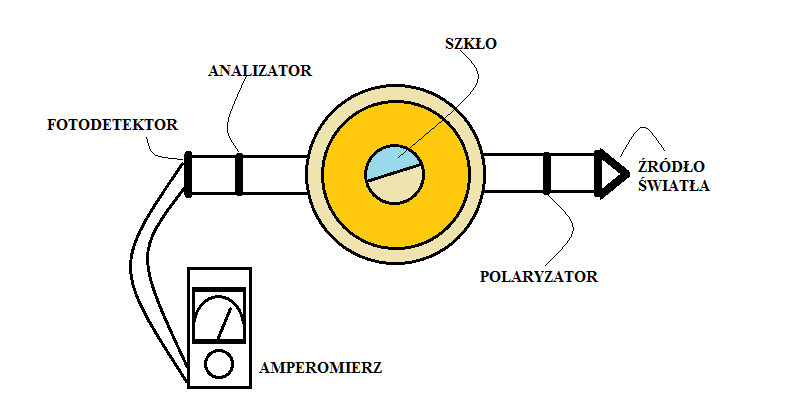
\includegraphics[width=17cm]{schemat3.png}
\section{Zadanie 1.}
\subsection{Wyniki pomiarów}
\begin{tabular}{|c|c|c|c|c|c|c|}
$\alpha_w[^\circ]$ & I & zakres & 1 działka & wynik & $u(I)$ & $u(\Theta)[^\circ]$ \\\hline
5 & 30 & 10mA & 0,2mA & 6 & 0,1702 & 4\\
10 & 32 & 10mA& 0,2mA& 6,4 & 0,1702 & 4\\
15 & 30 & 10mA& 0,2mA& 6 & 0,1702 & 4\\
20 & 30 & 10mA& 0,2mA& 6 & 0,1702 & 4\\
25 & 30 & 10mA& 0,2mA& 6 & 0,1702 & 4\\
30 & 28 & 10mA& 0,2mA& 5,6 & 0,1702 & 4\\
35 & 28 & 10mA& 0,2mA& 5,6 & 0,1702 & 4\\
40 & 26 & 10mA& 0,2mA& 5,2 & 0,1702 & 4\\
45 & 24 & 10mA& 0,2mA& 4,8 & 0,1702 & 4\\
50 & 22 & 10mA& 0,2mA& 4,4 & 0,1702 & 4\\
55 & 20 & 10mA& 0,2mA& 4,0 & 0,1702 & 4\\
60 & 18 & 10mA& 0,2mA& 3,6 & 0,1702 & 4\\
65 & 16 & 10mA& 0,2mA& 3,2 & 0,1702 & 4\\
70 & 10 & 10mA& 0,2mA& 2,0 & 0,1702 & 4\\
75 & 8 & 10mA& 0,2mA& 1,6 & 0,1702 & 4\\
80 & 6 & 10mA& 0,2mA& 1,2 & 0,1702 & 4\\
85 & 4 & 3mA & 0,05mA & 0,2 & 0,621 & 4\\
90 & 1,5 & 3mA& 0,05mA & 0,075 & 0,621 & 4\\
95 & 7 & 0,3mA & 0,005mA & 0,035 & 0,281 & 4\\
100 & 4 & 0,3mA& 0,005mA & 0,02 & 0,281 & 4\\
105 & 11,5 & 0,3mA& 0,005mA & 0,0575 & 0,281 & 4\\
110 & 3 & 3mA & 0,05mA & 0,15 & 0,621 & 4\\
115 & 5 & 3mA&  0,05mA& 0,25 & 0,621 & 4\\
120 & 8,5 & 3mA&  0,05mA& 0,42 & 0,621 & 4\\
125 & 11,5 & 3mA& 0,05mA & 0,575 & 0,621 & 4\\
130 & 15 & 3mA& 0,05mA & 0,75 & 0,621 & 4\\
135 & 18 & 3mA& 0,05mA & 0,9 & 0,621 & 4\\
140 & 21 & 3mA& 0,05mA & 1,05 & 0,621 & 4\\
145 & 23,5 & 3mA& 0,05mA & 1,175 & 0,621 & 4\\
150 & 25,5 & 3mA& 0,05mA & 1,275 & 0,621 & 4\\
\end{tabular}


\subsection{Wykres}
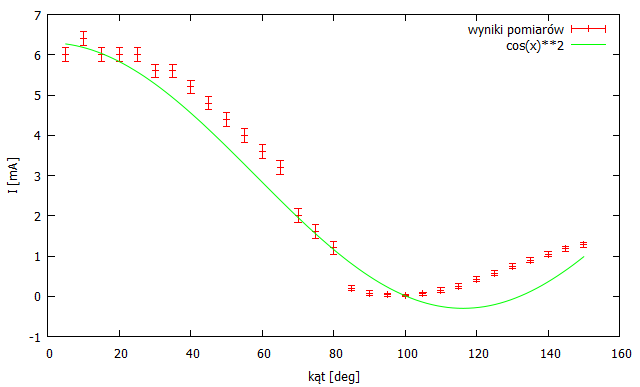
\includegraphics[width=15cm]{iodkat.png}
\subsection{Wnioski}
Różnice pomiędzy wynikami pomiarów a przewidywaniami teoretycznymi mogą być spowodowane występowaniem w obwodzie włączonej lampki oświetlającej biurko. Jednakowoż wyniki są podobne do przewidywań, co potwierdza prawo Malusa.
\section{Zadanie 2.}
\subsection{Wyniki pomiarów}
\begin{tabular}{|c|c|c|c|c|c|c|}
$\alpha[^\circ]$ & $\beta[^\circ]$ & $u(\beta)[^\circ]$ & $\sin(a)$ & $u(\sin(a))$ & $\sin(b)$ & $u(\sin(b))$ \\\hline
10 & 6 & 1 & 0,1736 & 0,0175 & 0,1045 & 0,0175\\
15 & 9 & 1 & 0,2588 & 0,0175 & 0,1564 & 0,0175\\
20 & 13 & 1 & 0,3420 & 0,0175 & 0,2250 & 0,0175\\
25 & 16 & 1 & 0,4226 & 0,0175 & 0,2756 & 0,0175\\
30 & 19 & 1 & 0,5000 & 0,0175 & 0,3256 & 0,0175\\
35 & 22 & 1 & 0,5736 & 0,0175 & 0,3746 & 0,0175\\
40 & 25 & 1 & 0,6428 & 0,0175 & 0,4226 & 0,0175\\
45 & 28 & 1 & 0,7071 & 0,0175 & 0,4695 & 0,0175\\
50 & 30 & 1 & 0,7660 & 0,0175 & 0,5000 & 0,0175\\
55 & 32 & 1 & 0,8192 & 0,0175 & 0,5299 & 0,0175\\
60 & 34 & 2 & 0,8660 & 0,0349 & 0,5592 & 0,0349\\
65 & 36 & 2 & 0,9063 & 0,0349 & 0,5878 & 0,0349\\
70 & 37 & 3 & 0,9397 & 0,0523 & 0,6018 & 0,0523\\
75 & 38 & 3 & 0,9659 & 0,0523 & 0,6157 & 0,0523\\
80 & 37 & 4 & 0,9848 & 0,0698 & 0,6018 & 0,0698\\
\end{tabular}
\subsection{Wykres}
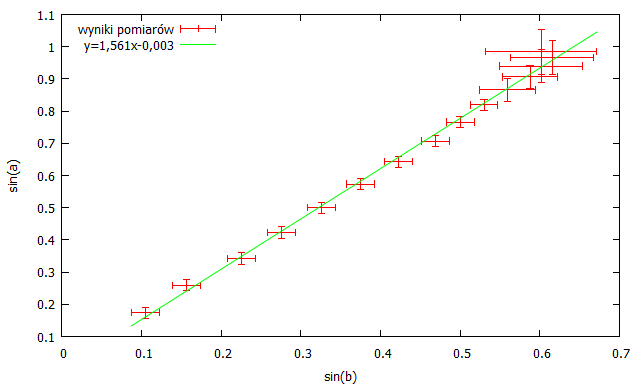
\includegraphics[width=15cm]{sinasinb.png}
\subsection{Obliczenia}
Szukaną wartość otrzymujemy stosując Metodę Najmniejszych Kwadratów minimalizując funkcję
\begin{equation}
	f(a,b) = \sum_{i=1}^n (ax_i+b-y_i)^2
\end{equation}
\begin{equation}
n_2 = \frac{\sin\alpha}{\sin\beta}=\text{ współczynnik kierunkowy prostej } +u(n_2) = 1,561 \pm 0,028
\end{equation} 
Ostatecznie
\begin{equation}
n_2 = 1,561 \pm 0,028
\end{equation} 
\section{Zadanie 3. - badanie kąta Brewstera}
\subsection{Wyniki pomiarów}
\begin{equation}
\alpha_\beta = 57^\circ
\end{equation} 
\begin{equation}
\beta = 33^\circ
\end{equation} 
\begin{equation}
\alpha_\beta + \beta = 90^\circ
\end{equation} 
\subsection{Obliczenia}
\begin{equation}
n_2 = \tg{\alpha_\beta}
\end{equation} 
\begin{equation}
n_2 = \tg{57^\circ} = 1,5398
\end{equation} 
\begin{equation}
u(n_2) = |\frac{u(\alpha_\beta)}{\cos^2{\alpha_\beta}} |= 0,117 
\end{equation} 
Ostatecznie
\begin{equation}
n_2 = 1,54 \pm 0,12
\end{equation} 
\section{Zadanie 4.}
\subsection{Wyniki pomiarów}
\begin{equation}
\alpha_{gr} = 43^\circ \pm 5^\circ
\end{equation} 
\subsection{Obliczenia}
\begin{equation}
n_2 = \frac{1}{\sin{\alpha_{gr}}} = 1,466279
\end{equation} 
\begin{equation}
u(n_2) = |\frac{-\cos{\alpha_{gr}}}{\sin^2{\alpha_{gr}}}\cdot u(\alpha_{gr})| = 0,14 
\end{equation} 
Ostatecznie
\begin{equation}
n_2 = 1.46 \pm 0,14
\end{equation} 
\section{Wnioski}
Ćwiczenie laboratoryjne miało na celu badanie zjawisk optycznych. Tematem przewodnim wykonywanych zadań była obserwacja odbicia światła od powierzchni dielektryka. Przeprowadzone doświadczenia pozwoliły nam pogłębić swoją wiedzę i poszerzyć horyzonty, potwierdzając prawa Malusa i Snelliusa, które stały się dla nas jasne po wcześniejszym wstępie teoretycznym.

Pomiary dały nam satysfakcjonujące wyniki, zgodne z przewidywaniami postawionymi dzięki teoretycznym przesłankom.
Niecałkowita zbieżność widoczna w zestawieniu powyższych danych może mieć podstawy w wielorakich czynnikach zewnętrznych, do których mogą należeć na przykład wpływ urządzeń laboratoryjnych niebędących częścią badanych układów (takich jak lampka oświetlająca stół), bądź niedokładnośc odczytu z urządzeń pomiarowych.

Doświadenia, które miały miejsce w Centralnym Laboratorium Fizycznym miały na celu także wyznaczenie \emph{kąta Brewstera}, dla którego odbita wiązka światła zanika i ustępuje miejsca efektowi wewnętrznego odbicia.

Wszystkie powyższe działania prowadziły jednak do innego szerzej zdefiniowanego celu, który przyświecał nam przez cały czas pracy, a mianowicie znalezienia współczynnika załamania światła badanego dielektryka. Udało nam się wyznaczyć tę wartość na trzy sposoby, z których najdokładniejszy okazał się ten wykorzystujący metodę Snelliusa.

\end{document}
 
